\documentclass[12pt,a4paper]{jarticle}

\usepackage{graphicx}
\usepackage{fancyhdr}
\usepackage{lastpage}
\usepackage{fancyhdr}
\usepackage{ascmac}
\usepackage[dvipdfmx]{graphicx}
\usepackage{here}
\usepackage{float}
\usepackage{framed}
\usepackage{array}
\usepackage[top=30truemm,bottom=30truemm,left=25truemm,right=25truemm]{geometry}
\pagestyle{fancy}
\lhead{\scriptsize Webプログラミング \quad -レポート課題 (第9回)-}
\rhead{\scriptsize 学籍番号:201711466 \quad 氏名:平井李音}
\cfoot{\thepage{}/{}\pageref{LastPage}}
\renewcommand{\thesection}{(\arabic{section})}
\renewcommand{\thesubsection}{\arabic{subsection}}

\begin{document}
\begin{ttfamily}

\section{アプリケーションの概要、特徴、工夫した点等の解説}
\subsection{概要}
このアプリケーションは、小説や漫画といった物語を作る上で、その世界特有の用語や登場キャラクターについてまとめるためのものです。
\subsection{特徴}
似たようなものとして@Wikiなどがあるが、それよりも簡単に編集が行える。
\subsection{工夫した点}
\subsubsection{パスワード}
作った世界、用語、キャラクターに任意でパスワードを設けることが出来る。
\par 世界にパスワードを設けることで、パスワードを知っている人だけに限定公開することが出来る。
\par 用語やキャラクターにパスワードを設けることで、勝手に内容を編集されることを防ぐことが出来る。


\section{ファイル間の関連、データ形式、プログラム等の解説}
\subsection{ファイル間の関連}
\begin{figure}[h]
  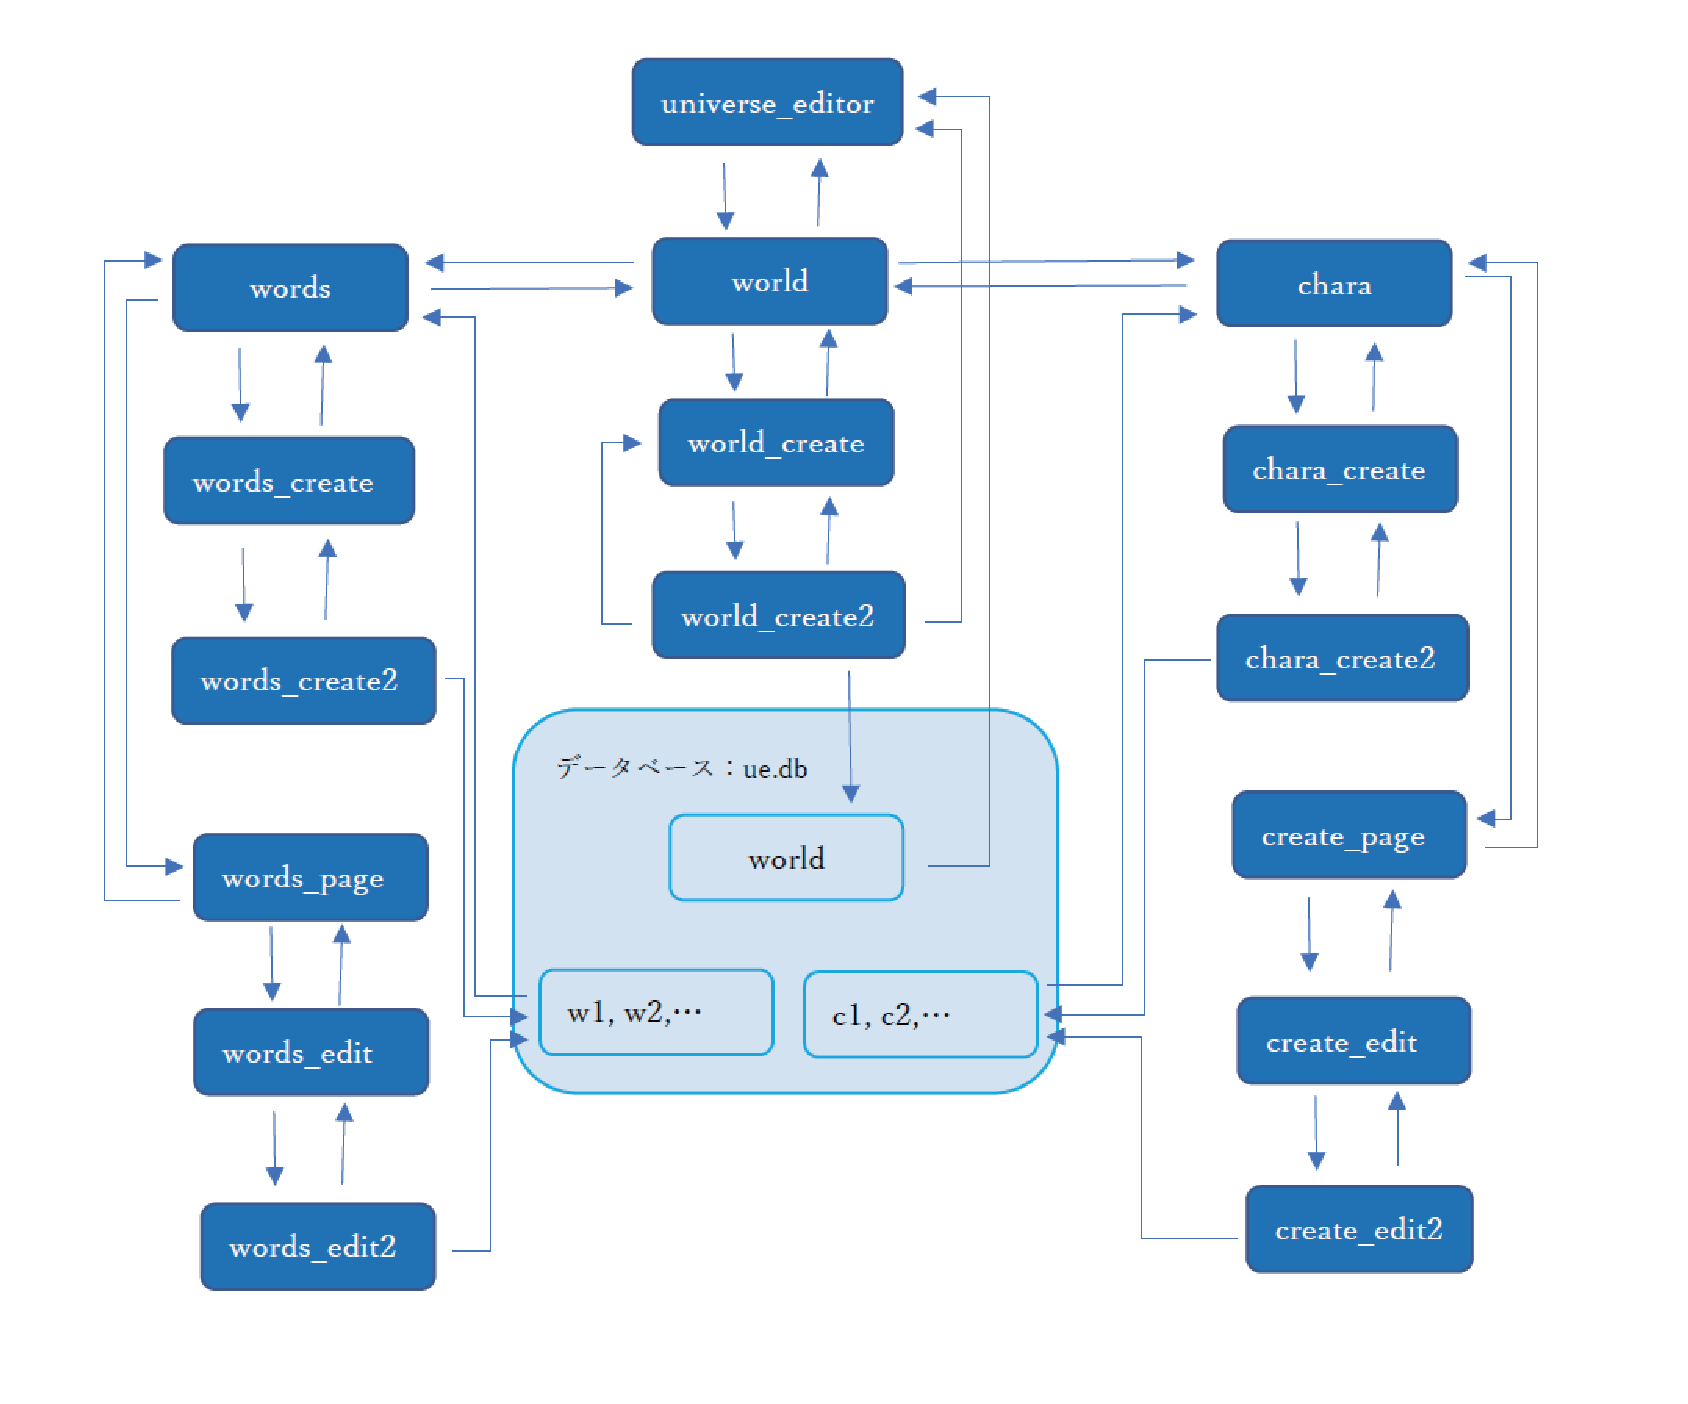
\includegraphics[width = 80mm]{10-2.eps}
  \centering
  \caption{ファイル間の関連}
\end{figure}
\subsection{データ形式}
使用しているデータは全て.db形式で保存している。
\subsection{プログラムの解説}
\subsubsection{}
\subsubsection{}
\subsubsection{}


\section{スクリーンショットを使った実行例とその説明}
\begin{figure}[htbp]
  \begin{center}
    \begin{tabular}{c}

      % 1 ホーム画面
      \begin{minipage}{0.53\hsize}
        \begin{center}
          \includegraphics[width=7.5cm]{07-01.eps}
          \hspace{1.6cm} [1]ホーム画面
        \end{center}
      \end{minipage}

      % 2 
      \begin{minipage}{0.53\hsize}
        \begin{center}
          \includegraphics[width=7.5cm]{07-02.eps}
          \hspace{1.6cm} [2]名前だけを入力した場合
        \end{center}
      \end{minipage}

      \begin{minipage}{0.55\hsize}
        \vspace{90mm}
      \end{minipage} \\
 
      % 3
      \begin{minipage}{0.53\hsize}
        \begin{center}
          \includegraphics[width=7.5cm]{07-03.eps}
          \hspace{1.0cm} [3]メッセージだけを入力した場合
        \end{center}
      \end{minipage}

      % 4
      \begin{minipage}{0.53\hsize}
        \begin{center}
          \includegraphics[width=7.5cm]{07-031.eps}
          \hspace{1.6cm} [4]HTMLタグを使った場合
        \end{center}
      \end{minipage}

    \end{tabular}
    \caption{動作している画面:エラーチェックの場合}
    \label{fig:dsplay}
  \end{center}
\end{figure}

\section{プログラムにアクセスするためのURL}
http://cgi.u.tsukuba.ac.jp/~s1711466/local_only/wp/universe_editor.rb

\section{授業の感想}



\end{ttfamily}
\end{document}
